%%%%%%%%%%%%%%%%%%%%%%%%%%%%%%%%%%%%%%%%%%%%%%%%%%%%%%%%%%%%%%%%%%%%%%%%%%%%%%%%
%2345678901234567890123456789012345678901234567890123456789012345678901234567890
%        1         2         3         4         5         6         7         8

\documentclass[letterpaper, 10 pt, conference]{ieeeconf}  % Comment this line out if you need a4paper

%\documentclass[a4paper, 10pt, conference]{ieeeconf}      % Use this line for a4 paper

\IEEEoverridecommandlockouts                              % This command is only needed if 
                                                          % you want to use the \thanks command

\overrideIEEEmargins                                      % Needed to meet printer requirements.
\pdfminorversion=4
\usepackage{graphics} % for pdf, bitmapped graphics files
\usepackage{epsfig} % for postscript graphics files
%\usepackage{mathptmx} % assumes new font selection scheme installed
%\usepackage{times} % assumes new font selection scheme installed
\usepackage{amsmath} % assumes amsmath package installed
\usepackage{amssymb}  % assumes amsmath package installed
\usepackage[nospace,sort]{cite}

%\usepackage{mathtools}
\usepackage{graphicx}
%\usepackage{subfig}
\newcommand{\vect}[1]{\mbox{\boldmath${#1}$}}%$
\newcommand{\mli}[1]{\mathit{#1}}

\title{\LARGE \bf
Reactive whole-body control for humanoid balancing on non-rigid unilateral contacts
}


\author{Mingxing Liu and Vincent Padois
\thanks{The authors are with}
\thanks{-Sorbonne Universit\'{e}, UPMC Univ Paris 06, UMR 7222, Institut des Syst\`{e}mes Intelligents et de Robotique, F-75005, Paris, France}
\thanks{-CNRS Centre National de la Recherche Scientifique, UMR 7222, Institut des Syst\`{e}mes Intelligents et de Robotique, F-75005, Paris, France}
\thanks{\tt\small \{liu, padois\}@isir.upmc.fr} }


\begin{document}
\maketitle
\thispagestyle{empty}
\pagestyle{empty}

\begin{abstract}
Humanoid robots are expected to act in human environments, where some of the contacts can be non-rigid. A fairly large amount of work has been devoted to the whole-body control of humanoids under rigid contacts, but few of them take into account non-rigid contacts. Indeed, the handling of unknown compliant contacts to achieve goal directed actions and whole-body balance remains a challenge. This paper addresses this problem by proposing a control mechanism that solves whole-body tasks under non-rigid contacts. It is a reactive control approach that automatically regulates contact forces and whole-body motions based on the motion of contact points without the awareness of the rigidity properties of the contact material. Verification of this approach is conducted through experiments on the iCub humanoid robot in simulation.
\end{abstract}


\section{Introduction}
Under-actuated robots, such as free-floating humanoid robots, usually need to make contacts with their environments to achieve some goal directed whole-body movements.
Most researches on whole-body control assume that the environment of a robot is rigid. This means that no adaptation to the environment compliance is needed for controllers. However, many objects in human environment can be  compliant (e.g. a soft cushion, a sofa, a yoga carpet). In this case, a controller that does not take into account the rigidity properties of the contact material is not sufficient. For example, pushing too strongly against a rigid object may result in damages to the robot or the environment; and pushing too weakly against a compliant object may not provide the robot with enough reaction forces to support its whole-body tasks. The problem becomes more complex when the rigidity of the object in contact is unknown a priori to robotic controllers, which is usually the case in many scenarios.
 
This paper aims at adapting whole-body motions of humanoid robots to unknown rigidity properties of the environment. This work is dedicated to whole-body balancing, and more generally whole-body control, with non-rigid, unilateral, frictional support contacts, for example, standing on a soft ground, or pushing against a compliant support contact with one hand while reaching for an object far away with the other hand (see Fig.\ref{reaching}). The problems of the manipulation of compliant objects and the handling of unexpected disturbance forces are beyond the scope of this paper. Moreover, the proposed control approach does not handle anticipatory aspects of balance, but it provides a reactive 
mechanism to maintain balance while multiple motion and contact tasks are being performed in a compliant environment.
\begin{figure}[!t]
\centering
\vspace{5pt}
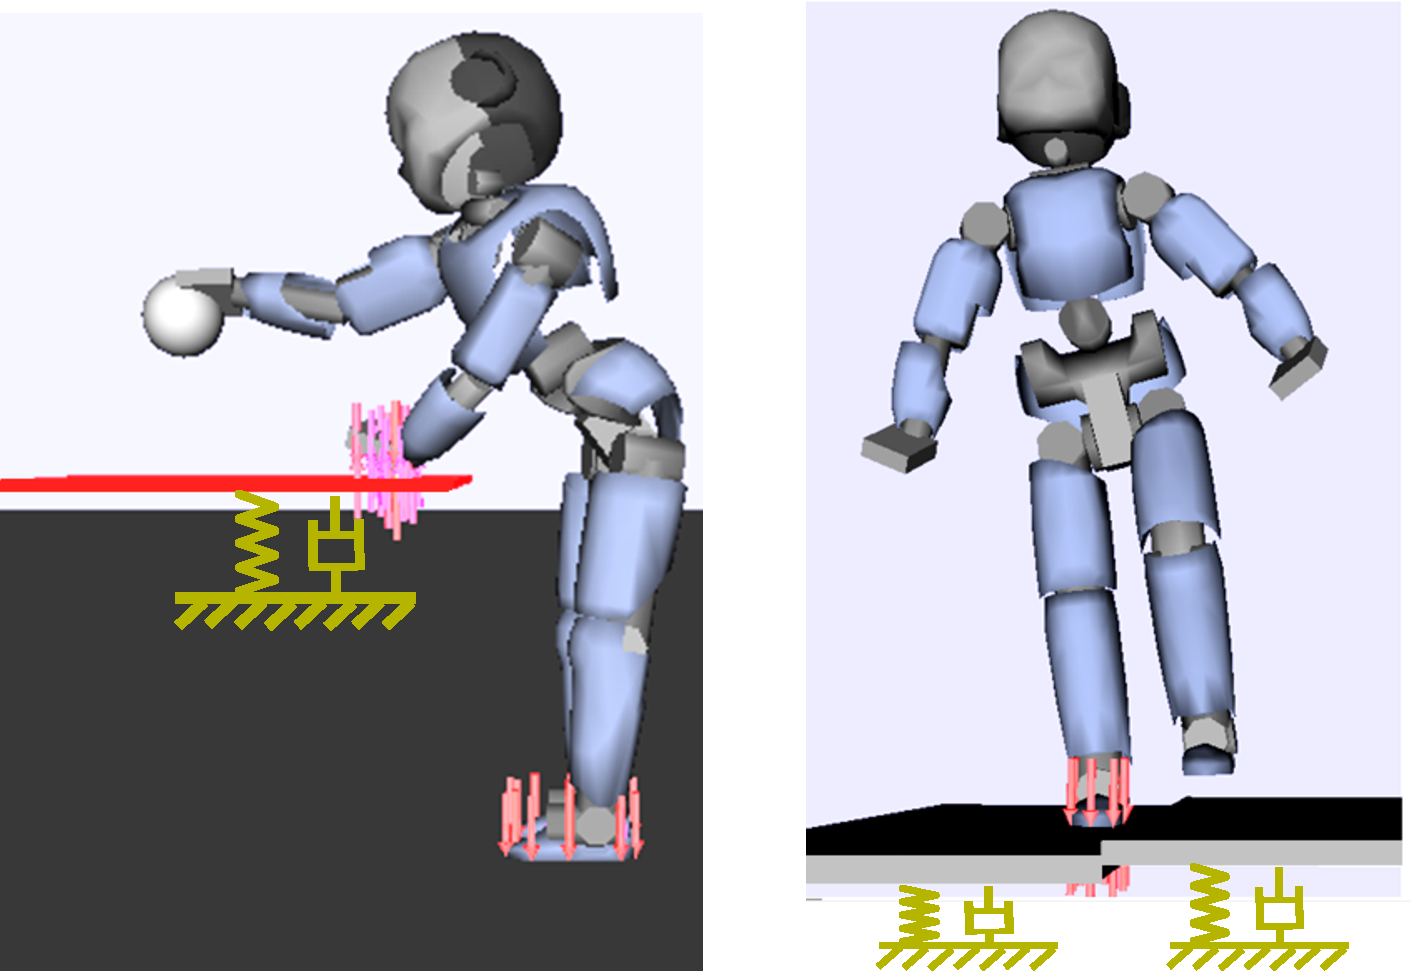
\includegraphics[width=.8\linewidth]{../figure/scenario.pdf}
\caption{Examples of balancing on non-rigid contacts during whole-body task execution.}
\label{reaching}
\end{figure}


\subsection{Related work}
The humanoid whole-body control problem has been addressed by different types of whole-body controllers, using analytical approaches \cite{Khatib08,Sentis10,Righetti13}, constrained quadratic programming \cite{Abe07,Liu11,Salini13,Saab13}, or a mixture of them \cite{Stephens10,Nori15}. These controllers are either developed for rigid environments, or validated only in rigid contact scenarios.
In general, a valid set of contact forces during whole-body task control can be found by solving a multi-objective problem with a set of elementary task objectives as well as constraints, such as whole-body dynamics, friction cone constraints for non-sliding contacts, and linear complementarity conditions \cite{Muico09,Saab13,Salini13}, which implies zero relative motions between two bodies in contact when normal contact force is non-negative. In the case of rigid contact with static environment, the linear complementarity condition implies two constraints: (i) the motion of the contact point is zero and (ii) the contact force along the normal to the contact surface is non-negative.  The zero motion constraint may not necessarily be true in the case of non-rigid contacts, since the velocities or accelerations of contact points may be non-zero, although the relative motion between the two contact points remains zero. In this case, hybrid control methods \cite{khatib87} that control forces and motions in orthogonal directions are not applicable. Therefore, the controller should take into account the dynamic relation between the contact point position and the contact force, rather than just control the contact force alone. 

Such physical interaction dynamics is taken into account in impedance control \cite{Hogan85} with the idea of controlling the relation between the contact point motion and the reaction force. Traditional impedance control \cite{Hogan85,Love95,Tsumugiwa02} computes the target impedance of the robot according to the estimated impedance of the environment, which requires high quality measurement of interaction forces. In \cite{Buchli10, Yang11}, learning approaches are applied to optimize the robot impedance. Such approaches do not require interaction force sensing and can be adaptable to variable environment impedance. However, the application of such approaches in the context of humanoid balance control with non-rigid contacts is not suitable. First, these methods rely on trajectory-based learning and adaptation algorithms, whereas there is not necessarily a reference motion trajectory for each support contact in the whole-body balancing context considered here. Furthermore, they need to explore the entire state-action space if a globally optimal solution is to be found, which is impossible for high dimensional robots such as humanoids.

The problem of humanoid balance control with deformable contact support was addressed in \cite{Bouyarmane11b}, which proposed a posture planning approach assuming that the contact material properties are known. A difference of the present paper with respect to \cite{Bouyarmane11b} is that the approach proposed here does not require the knowledge of the rigidity of the environment, and the controller works online in a reactive way.

\subsection{Contribution}
The contribution of this work consists in a reactive controller for whole-body balancing of humanoid robots performing whole-body tasks in unknown compliant environments. As the motions and forces at support contacts are related to whole-body task executions, their reference trajectories are unavailable a priori. Therefore, this approach focuses on the regulation of contact forces in a reactive way. It reacts to the motions of non-rigid contacts in real-time during whole-body movements, with the aim of establishing contact equilibrium quickly. 

A frictional non-rigid contact model is proposed (Section \ref{Section:modeling}) both for simulation and for control. The model parameters of the non-rigid environment are unknown to the controller. The force regulation approach does not try to estimate the impedance parameters of the environment, but it regulates contact forces by reacting to environment motions directly. This reactive control approach is embedded in an optimization based multi-task controller (Section \ref{Section:control}), which has been used to achieve whole-body control of humanoid robots in rigid environments. However, the reactive principle of the approach proposed here is general and can also be applied in many other whole-body controllers to handle non-rigid support contacts. Examples using this approach are provided in Section \ref{Section:Results}, where a humanoid robot performs reaching and stepping actions in a non-rigid environment. Further research directions related to this approach are presented in Section \ref{Section:Conclusions}.
 

\section{Contact Modeling}
\label{Section:modeling}
This work considers the handling of non-rigid support contacts. The environment is assumed to be passive and the contact surface at each contact point is supposed to be flat. The direction perpendicular to the contact surface and pointing towards the robot is denoted by $\vect{n}$. The interaction force exerted by the robot on the environment is $\vect{F}=[\vect{F_t}^T, \vect{F_n}^T]^T$, with $\vect{F_t}$, the tangential contact force and $\vect{F_n} = -F_n\vect{n}$, the normal force (the component perpendicular to the contact surface).  

The dynamics of a non-rigid environment here is modeled as a mass-spring-damper system as shown in Fig. \ref{contact_model}. A rigid mass is attached to a massless spring with spring constant $k$ and a massless viscous damper with constant $d$. In the model used here, the mass only moves along the directions $\vect{n}$ or $-\vect{n}$. The position of the contact point along $\vect{n}$ is denoted as $\vect{p}=p\vect{n}$. The normal velocity of the contact point with respect to the world frame $\mathcal{W}$ is denoted as $\vect{v_n}$.
The length of the spring is limited.
When the spring is not completely compressed, the magnitude of the normal contact force exerted by the robot on the environment is 
\begin{equation}
\vect{F}_n = m\ddot{\vect{p}}+k \Delta \vect{p} +d\dot{\vect{p}}, 
\ \text{with} \ \left\|\Delta \vect{p}\right\| \leq \Delta p_{max}
\end{equation} 
where  $\Delta \vect{p} = \vect{p} - \vect{p}_0$ is the displacement of the mass with respect to its rest position $\vect{p}_0$, and $\Delta p_{max}$ is the limit amount of the displacement. 
When the spring is completely compressed, the contact becomes rigid.
For the contact to exist, the normal contact force must be non-negative: $F_n\geq 0$, because the contact point of the robot can only push the mass but not pull it (unilateral contact). 


To ensure a non-sliding contact, the frictional contact force is constrained to lie within the Coulomb friction cone: $\mathcal{C} = \left\{\vect{F} \mid \left\|\vect{F_t}\right\|\leq \mu \left\|\vect{F_n}\right\|\right\}$, where $\mu>0$ is the friction coefficient at the contact point. The friction cone is usually approximated by a \textit{k}-faced convex polyhedron so that the non-sliding contact constraint can be formulated as a linear constraint.
\begin{figure}[!t]
\centering
\vspace{5pt}
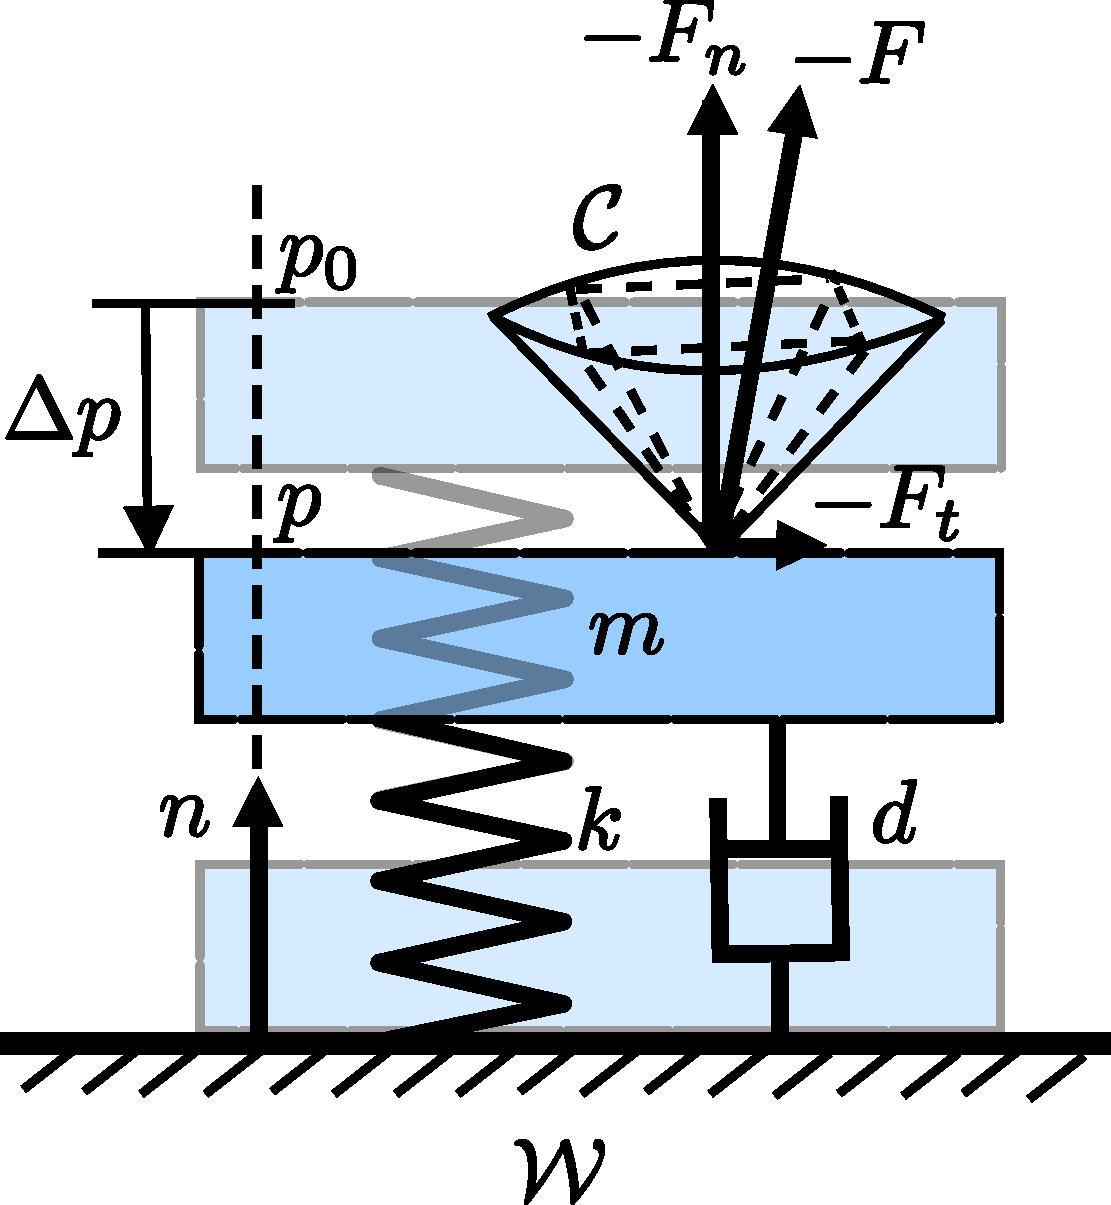
\includegraphics[width=0.6\linewidth]{../figure/mass_spring_damper.pdf}
\caption{Modeling of a frictional non-rigid contact with a mass spring damper system and Coulomb's friction cone.}
\label{contact_model}
\end{figure}

\section{Reactive Whole-Body Control under Non-Rigid Contacts}
\label{Section:control}
The reactive whole-body control proposed here solves a set of elementary operational tasks as well as constraints to ensure whole-body balance during task execution. An elementary operational task considered here can be either a motion task (e.g. center of mass motion task, hand motion task, foot motion task, posture task, etc.), or a contact task (hand contact task, foot contact task, etc.). Especially, the above-mentioned contact model is used here to adapt whole-body movements to frictional non-rigid support contacts. The whole-body control of all the tasks and constraints are formulated as a Linear Quadratic Programming (LQP) problem \eqref{lqp}. The output of this LQP problem is the optimal joint accelerations $\ddot{\vect{q}}$, joint torques $\boldsymbol{\tau}$, and contact forces $\vect{F}$.

\begin{subequations}
\label{lqp}
\begin{eqnarray}
\mathop{{\arg\min}\vphantom{\sim}}\limits_{\substack{\ddot{\vect{q}},\boldsymbol{\tau},\vect{F}_c}}
&\sum\limits_{i}\left\Vert J_i(\vect{q})\ddot{\vect{q}} + \dot{J}_i(\vect{q})\dot{\vect{q}} - \ddot{\vect{p}}_{i}^d \right\Vert^2_{Q_i} \label{obj1}\\
&+ \sum\limits_{c}\left\Vert \vect{F}_c - \vect{F}_c^d \right\Vert_{Q_c}^2 \label{obj2}\\
&+ \left\Vert \boldsymbol{\tau} \right\Vert_{Q_r}^2 + \left\Vert \ddot{\vect{q}} \right\Vert_{Q_r}^2\label{obj3}\\ 	
 \text{s.t.} & M(\vect{q})\ddot{\vect{q}} + \vect{b}(\vect{q},\dot{\vect{q}})= S^{T}\boldsymbol{\tau} - \sum\limits_{c}J_{c}(\vect{q})^{T}\vect{F}_c\label{c1}\\
&  \vect{F}_c \in \mathcal{C}_c \label{c2}\\
& \underline{\vect{F}_c}\leq \vect{F}_c \leq \overline{\vect{F}_c}\label{c3}\\
& \underline{\boldsymbol{\tau}}\leq \boldsymbol{\tau} \leq \overline{\boldsymbol{\tau}}\label{c4}\\
& \underline{\vect{q}}\leq \frac{1}{2}\ddot{\vect{q}}\delta t^2 + \dot{\vect{q}}\delta t + \vect{q} \leq \overline{\vect{q}}\label{c5}
\end{eqnarray}			  
\end{subequations}
where several task objectives are optimized subject to the whole-body dynamics constraint \eqref{c1}, the friction cone constraint \eqref{c2}, bounds on contact forces \eqref{c3}, joint torque limits \eqref{c4}, and joint limits \eqref{c5}.
$M(\vect{q})$ is the generalized inertia matrix.
$\dot{\vect{q}}$ and $\ddot{\vect{q}}$ are the vector of velocity and the vector of acceleration in generalized coordinates, respectively.
$\vect{b}(\vect{q},\dot{\vect{q}})$ is  the vector of Coriolis, centrifugal and gravity induced joint torques.
$S$ is a selection matrix for the actuated degrees of freedom (DoF).
Joint limit constraint \eqref{c5} is expressed with respect to joint accelerations based on a discrete linear approximation of joint positions with a time step of $\delta t$.

Objective \eqref{obj1} minimizes the error of task acceleration for elementary motion task control.
Each motion task $i$ is associated with a local proportional-derivative (PD) controller $\ddot{\vect{p}}_{i}^d=K_{p,i}\vect{e}_i + K_{d,i}\dot{\vect{e}}_i$. The inputs of this PD controller are task position and velocity errors ($\vect{e}_i$ and $\dot{\vect{e}}_i$), and the output is the desired acceleration $\ddot{\vect{p}}_{i}^d$ of the controlled frame. Here $K_{p,i}$ and $K_{d,i}$ are symmetric, positive definite gain matrices, $J_i$ is the task Jacobian, and $Q_i$ is a diagonal weighting matrix to regulate the importance level of task $i$. 

%Objective  \eqref{obj2} handles contact forces.
%Each contact task $c$ is associated with a contact force variable $\vect{F}_c$. 
As the contact force $\vect{F}_c$ affects the whole-body motion, its appropriate value should be computed in consideration of all the tasks to be performed and constraints to be met. There are actually  infinite contact force solutions that satisfy all these task objectives and constraints. The regularization task \eqref{obj2} can be used to ensure the uniqueness of the solution by mimizing the norm of $\vect{F}_c$. Indeed, as mentioned in \cite{Liu11}, one can set the value of desired contact force $\vect{F}_c^d$ in \eqref{lqp} to zero, set the weight $Q_c$ to a low value compared to $Q_i$, and let the optimization to compute the appropriate value of $\vect{F}_c$.  
However, in this work, which deals with non-rigid contacts,  $\vect{F}_c^d$ is computed according to the local contact information, in order to speed up robot reaction to non-rigid contacts. This computation of $\vect{F}_c^d$ is described in \ref{balance}. This desired contact force is used to guide the search of the optimal contact force in optimization \eqref{lqp}, and the suitable value of $\vect{F}_c$ is still provided by \eqref{lqp} to satisfy all the constraints in \eqref{lqp}.

Objective \eqref{obj3} is a regulation term that minimizes the norms of the variables $\boldsymbol{\tau}$ and $\ddot{\vect{q}}$. This objective is useful for ensuring the uniqueness of the solution for redundant robots. As this objective may increase the errors of other elementary tasks, its weight $Q_r$ is set to a very low value compared to other objective weights. 
The whole reactive whole-body control system is summarized in Fig. \ref{schema}.
\begin{figure}[!t]
\centering
\vspace{5pt}
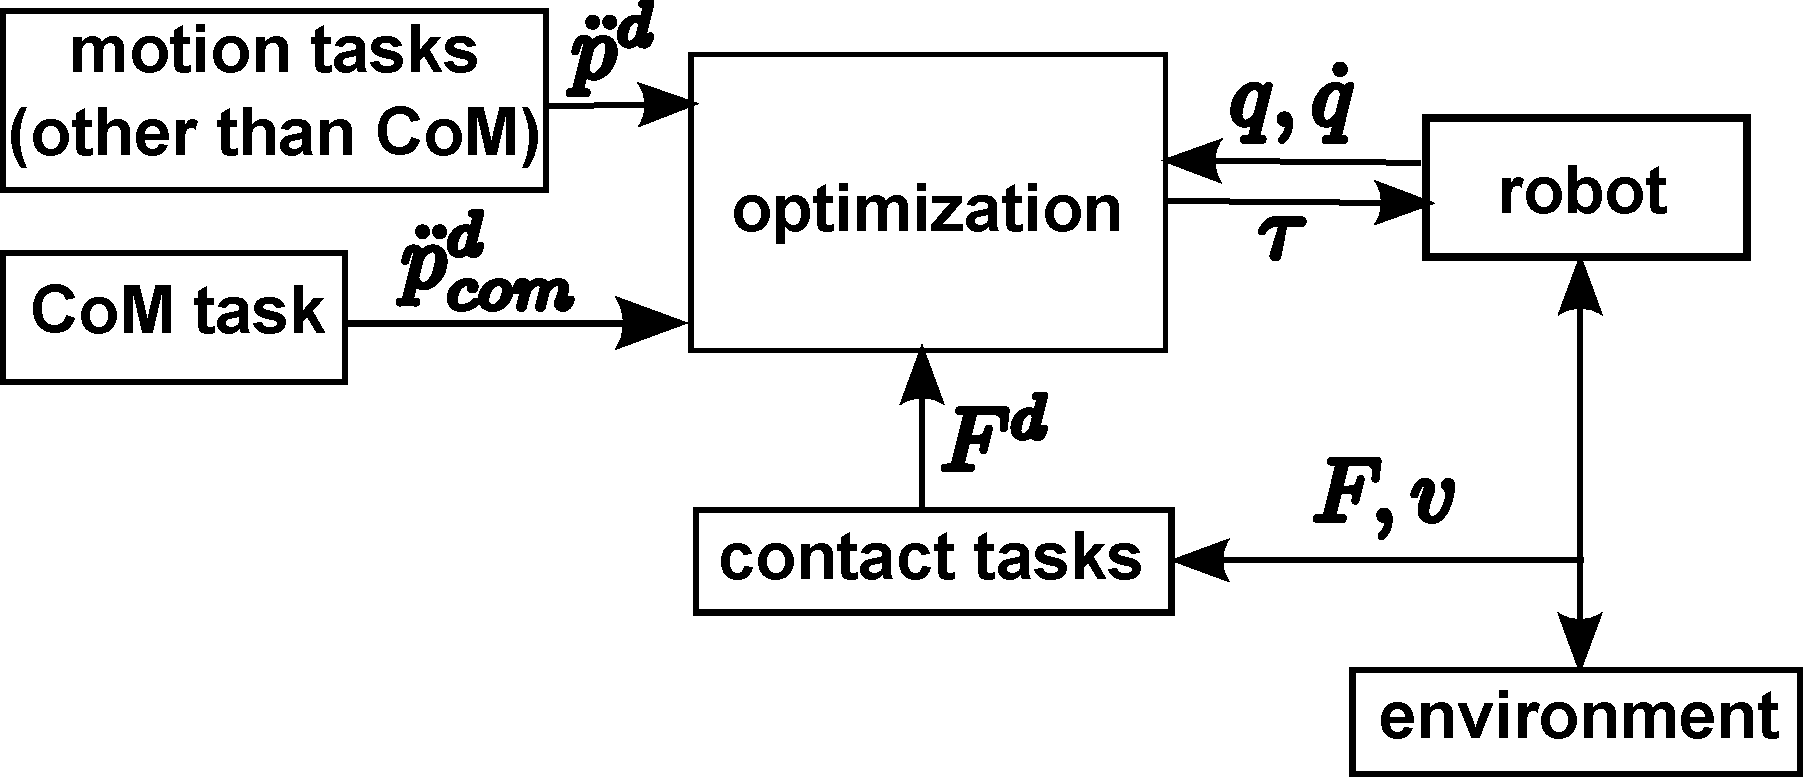
\includegraphics[width=.8\linewidth]{../figure/schema.pdf}
\caption{Block schema of the whole reactive whole-body control system.}
\label{schema}
\end{figure}

\subsection{Handling of interaction force at non-rigid support contact}
\label{balance}
In this work, a multi-contact state is supposed to be in static equilibrium if there is no motion at support contacts.
Take the reaching scenario shown in Fig. \ref{reaching} for example, if the support hand pushes too slightly against the table surface, the reaction force generated by the table is too weak to support the robot's leaning posture, and the robot may not be able to provide enough joint torques to maintain its posture. In this case, the contact is not in equilibrium as the support hand will keep sinking with the table surface.
If the hand pushes strongly enough, the contact equilibrium may be established.
However, the multi-contact system usually does not have a unique equilibrium state due to the redundancy of the system.   
In the reaching scenario, three situations can be listed when the robot leans forward to reach for an object:
\begin{enumerate}
	\item if the hand contact force is weak, the robot may have to strengthen a lot in order to maintain the leaning posture.
	\item If the hand pushes the table more strongly, a sufficient reaction force is generated by the supporting surface to maintain the leaning posture, and the robot does not have to strength a lot to maintain contact equilibrium.
  \item If the hand pushes the table too strongly, the robot may have to strengthen a lot again in order to balance internal forces created by hand contact force to maintain equilibrium.
\end{enumerate}
As there is a wide range of hand contact forces that can satisfy the equilibrium of the multi-contact system, it is desirable to find appropriate contact forces to rapidly achieve an equilibrium state in a natural way. Therefore, in addition to the optimization of contact forces by a comprehensive consideration of all the task objectives and constraints in \eqref{lqp}, the desired contact force is adapted to local contact information. Indeed, as long as the contact point is moving along the pushing direction, the robot cannot rely on this contact point to maintain its equilibrium and the desired contact force will be kept increased until the material is sufficiently compressed and no more movement is produced at the contact point ($\vect{v}_c=\vect{0}$). In this way, the contact equilibrium is attained rapidly and the contact point can fully support the whole-body task execution.

The regulation of the desired contact force depends on the rigidity of contact materials. Although the contact material is unknown a priori, the robot can adapt its rigidity by pushing against it. Here the approach does not estimate the parameters of a  model of the environment, but it does regulate the contact force in a reactive way.  The idea is to first apply a small amount of pushing force $\underline{\vect{F}_c}$ at the beginning of contact ($\vect{F}_c^d(t_0)=\underline{\vect{F}_c}$) to activate it. If the contact surface is soft, then it starts to move along the pushing direction ($\vect{v}_c>\vect{0}$). Afterward, the variation of desired contact force $\delta\vect{F}_c$ is computed at each time step during the pushing action. 

The form of $\delta\vect{F}_c$ can be chosen by an analysis of the energy variation during the pushing action\footnote{It is assumed here that the impedance of the robot itself remains high with respect to the impedance of the contact surface and that the energy is mostly dissipated by the non-rigid environment.}. At time $t=t_l$, the kinetic energy of the local interaction system is $\frac{1}{2}m_c(t_l) \left\Vert\vect{v}_c(t_l)\right\Vert^2$, where $m_c$ is the equivalent mass of the robot-environment system at contact point $c$. Part of this energy is supposed to be absorbed by the spring displacement $\Delta \vect{p}$, with the rest being dissipated by the damper after a short amount of time $\Delta t$
\begin{equation}
\frac{1}{2}k\Delta \vect{p}^2 + \int_{t_l}^{t_l+\Delta t} d \left\Vert\vect{v}_c(t)\right\Vert^2 \mathrm{d}t =  \frac{1}{2} m_c(t_l) \left\Vert\vect{v}_c(t_l)\right\Vert^2.\label{energy}
\end{equation}
Substituting the total variation of the spring force from $t_l$ to the end of pushing
$\Delta \vect{F}_c = k\Delta \vect{p}$ in \eqref{energy} leads to
\begin{equation}
\left\Vert\Delta \vect{F}_c\right\Vert = \frac{m_c(t_l) \left\Vert\vect{v}_c(t_l)\right\Vert^2 -2\int_{t_l}^{t_l+\Delta t} d \left\Vert\vect{v}_c(t)\right\Vert^2 \mathrm{d}t}{\left\Vert\vect{v}_c(t_l)\right\Vert\Delta t}.
\end{equation}
Supposing $\vect{v}_c$ is constant from $t_l$ to $t_l+\Delta t$, the order of magnitude of $\left\Vert\Delta \vect{F}_c\right\Vert$ can be estimated to be $\left(\frac{m_c(t_l)}{\Delta t}-2d\right)\left\Vert\vect{v}_c(t_l)\right\Vert$.
This extra amount of spring force needs to be balanced by extra robot contact forces finally to maintain contact equilibrium.
In fact, the increase of the contact force at each time step may result in the increase of the contact point velocity towards the pushing direction, thus it may accelerate the pushing action until the material is completely compressed with respect to the whole-body motion of the robot.
Based on the above analysis, the desired contact force variation can have the same order of magnitude as $\Delta \vect{F}_c$ does, which is proportional to $\vect{v}_c(t_l)$.
Therefore, the desired contact force $\vect{F}_c^d(t_l)$ can be computed as follows 
\begin{equation}
\begin{aligned}
&\vect{F}_c^d(t_l) = \vect{F}_c(t_{l-1}) + \delta\vect{F}_c(t_l) \label{fc}\\
&\text{with}\ \delta\vect{F}_c(t_l) = a(t_l) \vect{v}_c(t_l),
\end{aligned}
\end{equation}
 where $a(t_l)$ is a non-negative parameter. A large value of $a$ corresponds to a small value of $\Delta t$, which implies a faster pushing action. To avoid abrupt changes in the contact force, the value of $\delta\vect{F}_c$ is bounded. Moreover, for safety reason, the contact force is limited by its upper bound $\overline{\vect{F}_c}$ in \eqref{c3} to prevent the robot from pushing too strongly when it touches a very rigid surface at the end of the pushing action.
 
% This choice is due to the fact that the softer the contact surface is (with a weaker stiffness $k$ and a weaker damping $d$), the faster it tends to move along the pushing direction under a pushing force. In this case, the robot can further compress the object by the increase of contact force until it obtains a reaction force that is strongly enough to support its whole-body posture. 

\subsection{Center of mass control}
\label{Subsec:com_control}
During a quasi-static movement, the position of center of mass (CoM) plays an important role in balance control. For fixed contact point placements, the CoM must lie above the projection of a convex set that is defined by the properties of each contact placement \cite{Bretl08}.
In many applications, the CoM target position is given a priori. For example, it is usually fixed above the center of support polygon when the robot is standing, or planned by predictive control for locomotion \cite{Wieber06}. Moreover, the CoM task is usually assigned with a high priority with respect to contact force related tasks (not contact constraints) to ensure balance. In this case, the CoM position may dominate the control of contact forces. For example, no matter what desired contact force is assigned to a foot contact task of a standing robot, its real value will be governed by the motion of the CoM. However, the desired CoM position planned a priori may not be suitable in a non-rigid environment, because the planner cannot take into account the unknown rigidity of the contact surface. Therefore, the planned CoM target position is adjusted here to adapt to the compliance of the environment, or in other words, to the desired contact forces at non-rigid support contacts. 

The adaptation of the CoM position is based on a simplified model of the robot, including a punctual mass ($m$) at the CoM linked to several massless legs or arms.
This simplified model is in static equilibrium under desired contact forces $\vect{F}_c^d$ if 
%the force and moment equilibrium under the gravity force and all the contact forces is maintained and each contact force lies in a friction cone.
\begin{subequations}
\label{equilibrium}
\begin{eqnarray}
&\sum\limits_{c}\vect{F}_c^d + m\vect{g} = \vect{0} \label{equilibrium1}\\
&\sum\limits_{c}\vect{p}_c\times\vect{F}_c^d + \vect{p}_{com}\times m\vect{g}= \vect{0} \label{equilibrium2}\\
&\vect{F}_c \in \mathcal{C}_c, \label{equilibrium3}
\end{eqnarray}
\end{subequations}
where $\vect{F}_c^d$ is computed in \eqref{fc}, $\vect{g}$ is gravity acceleration, $\vect{p}_c$ is the position of contact point $c$, and $\vect{p}_{com}$ is the CoM position.
Condition \eqref{equilibrium3} is momentarily neglected here since it is accounted for when solving \eqref{lqp}.
The other two conditions \eqref{equilibrium1} and \eqref{equilibrium2} allow us to compute $\vect{p}_{com}^d$ compatible with $\vect{F}_c^d$ by solving 
\begin{equation}
\label{pcom}
\sum\limits_{c}\vect{p}_c\times\vect{F}_c^d - \vect{p}_{com}^d\times \sum\limits_{c}\vect{F}_c^d= \vect{0}.
\end{equation}
It can be proved that the components of $\vect{p}_{com}^d$ in the plane of contact surface can always be found by solving \eqref{pcom}, as long as the contact forces along the normal direction are constrained to be non-zero, which can be ensured by setting $\underline{\vect{F}_c}>\vect{0}$ in \eqref{c3}.
Note that $\vect{p}_{com}^d$ is computed to be adaptable to $\vect{F}_c^d$ but with \eqref{equilibrium3} neglected. Therefore, to ensure equilibrium for the robot, the adapted CoM target position $\vect{p}_{com}^d$ should be further constrained within its admissible domain defined by \eqref{equilibrium}, which can be obtained by using the approach described in \cite{Bretl08}.

\section{RESULTS}
\label{Section:Results}
The reactive whole-body control proposed in section \ref{Section:control} is applied here to handle multiple non-rigid contacts during whole-body task execution.
The approach is applied to a $38$-DoF free-floating iCub robot in the simulator XDE \cite{Merlhiot12}, which is a software environment that manages physics realistic simulation.
Some example applications of the proposed approach can be seen in the video attached to this paper. These applications are: reaching with one hand supported by tables of different degrees of rigidity and stepping on a soft floor.
 

\subsection{Reaching with one hand supported by a soft table}
In this scenario, the robot is standing on the ground and reaching for an object above a table with its right hand. As the object is far away, its left hand is in contact with the table to obtain an additional support that increases its reaching ability (see Fig. \ref{reaching_table}). The non-rigid table is modeled using the model described in \ref{Section:modeling}. 
The controlled motion tasks include the 2-D CoM position task, 6-D the right hand position and orientation task, the 32-D posture task, and the 1-D head position task. The right hand target position is the object above the table. The posture task tries to keep the body upright. The contact tasks handle the left hand contact with the table and eight foot contacts with the ground. Each contact force is constrained to lie inside a friction cone to avoid slippage. The maximum magnitudes of the hand contact force $\overline{\vect{F}_c}$ and of its variation $\overline{\delta \vect{F}_c}$ are set to $50N$ and $1.5N$, respectively. The minimum contact force $\underline{\vect{F}_c}$ is set to $2N$ to keep the contact active.
\begin{figure}[!t]
\centering
\vspace{5pt}
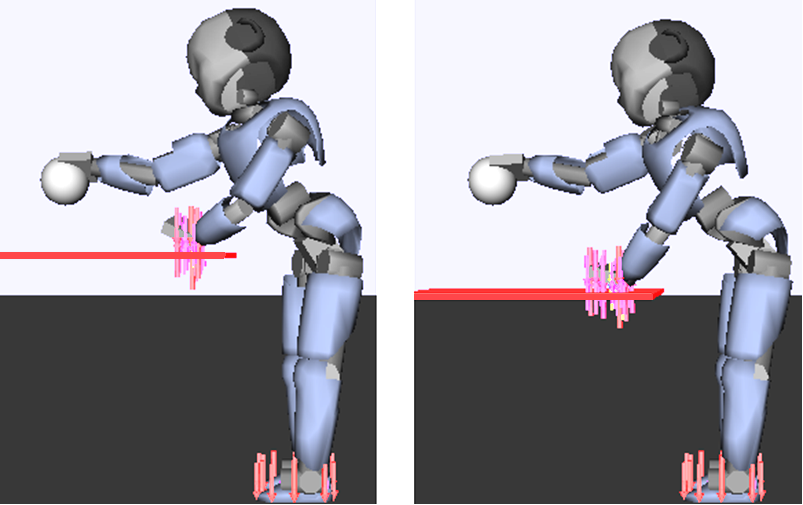
\includegraphics[width=.75\linewidth]{../figure/reaching_different_k2.png}
\caption{Snapshots of the robot reaching with one hand supported by a table. The table on the right is softer than the one on the left.}
\label{reaching_table}
\end{figure}

In this experiment, different degrees of rigidity of the table are tested, from a very soft case to a nearly rigid case. In all these tests, the robot is able to adapt the pushing behavior of the left hand, and the right hand successfully reaches the goal.
The resulting hand contact force ($\vect{F}_c$) as well as its desired variation ($\delta\vect{F}_c$) is shown in Fig. \ref{reaching_force}, with the coefficient $a$ set to $5 Ns/m$.
\begin{figure}[!t]
\centering
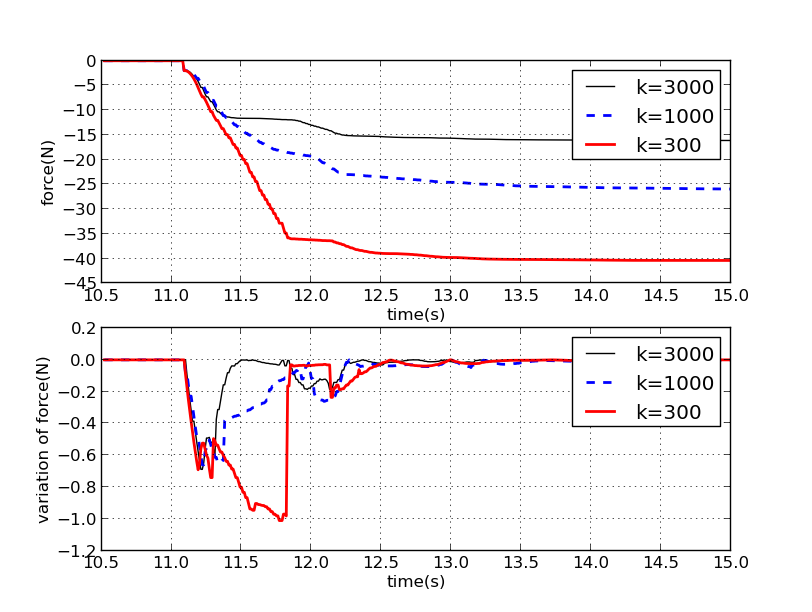
\includegraphics[width=\linewidth]{../figure/force_k300-3000_d5.png}
\caption{The contact force between the left hand and the table (above) and the variation of desired contact force (below). The stiffness of the table is modified, from $k=300 N/m$ to $k=3000 N/m$, the contact point displacement is limited by $\Delta p_{max} = 5 cm$, and $d$ is set to $2\sqrt{k}$.}
\label{reaching_force}
\end{figure}

\begin{figure}[!t]
\centering
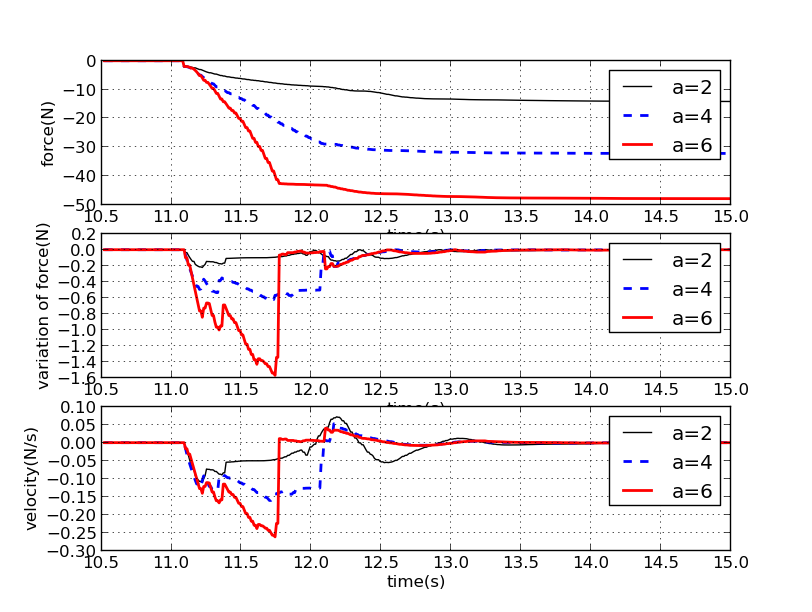
\includegraphics[width=\linewidth]{../figure/velocity_k300_d2-6.png}
\caption{The contact force between the left hand and the table (above), the variation of desired contact force (middle), and the hand velocity (below). The stiffness of the table is $k=300 N/m$, and $a$ is changed from $2 Ns/m$ to $6 Ns/m$. A larger $a$ results in stronger contact force, but establishes contact equilibrium faster; while a smaller $a$ provides weaker support force, resulting in more fluctuation of velocity during whole-body task execution.}
\label{reaching_velocity}
\end{figure}
This figure shows that the hand contact force converges no matter if the table surface is soft ($k=300 N/m$) or hard ($k=3000 N/m$). When the table is soft, larger force variations are generated during the pushing action in order to establish contact equilibrium quickly. The softer the table is, the stronger the resulting contact force becomes. This is logical since the soft table displaces easily while being pushed, so that the hand sinks together with the table, making the body lean forward more. Thus more reaction force is needed from the table to support the bended posture. 
%1) The robot fails as it did not compensate for the unexpected dynamics of the soft table surface.

The role of $a$ is to regulate the ratio of force variation with respect to contact point velocity. In Fig. \ref{reaching_velocity}, contact forces as well as contact point velocity with respect to different values of $a$ and the same table stiffness ($k=300 N/m$) are shown. It can be seen that a larger $a$ makes the contact point sinks faster, resulting in stronger contact force, but making the velocity converges to zero faster; while a smaller $a$ provides weaker support force, resulting in more fluctuation of velocity during whole-body task execution.
The choice of the value of $a$ depends on how quickly the equilibrium is desired to be established. However, a too large $a$ may result in too large force variation. Therefore, the magnitude of the force variation is bounded here to avoid large peaks in contact forces.

The computation time for the proposed control algorithm for this experiment is presented in Figure \ref{computation_cost}.
\begin{figure}[htbp]
\centering
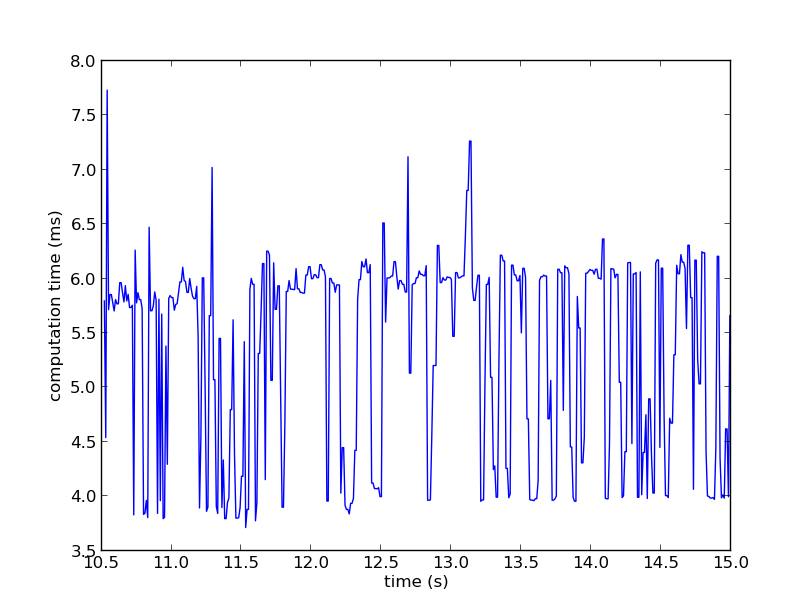
\includegraphics[width=\linewidth]{../figure/consum.png} 
\caption{\label{computation_cost} Computation time for the control algorithm.}
\end{figure}
It can be seen in Figure \ref{computation_cost} that for the iCub robot with $38$ DoF performing $13$ motion and force tasks, and with a total task dimension of $68$, the computation time for the control algorithm is within $10 ms$ without any specific code optimization. Real time implementation of the proposed approach on a torque controlled humanoid robot can thus be envisioned.

\subsection{Stepping on a soft floor}
In this experiment, the robot keeps switching its stance foot on a soft floor (see Fig. \ref{walking}). The soft floor is modeled as two separate movable planks, one under each foot.
\begin{figure}[!t]
\centering
\vspace{5pt}
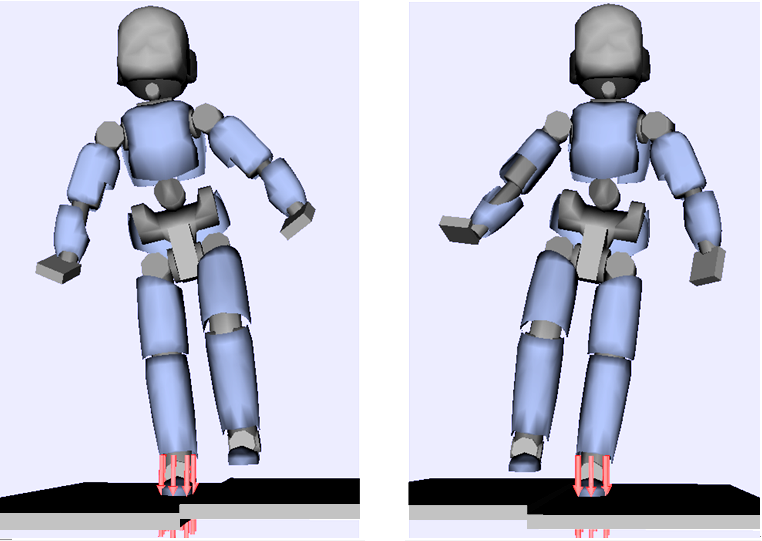
\includegraphics[width=.75\linewidth]{../figure/switch_contact_foot2.png}
\caption{Snapshots of the robot stepping on a soft floor.}
\label{walking}
\end{figure}
The controlled tasks include the CoM task, the moving foot task, the posture task, and the stance foot contact task. Each foot contact force is constrained to lie inside a friction cone to avoid foot slippage. As mentioned in section \ref{Subsec:com_control}, instead of manually switching the CoM target position between above the two feet, it is computed automatically based on the desired foot contact force by solving \eqref{pcom}. 

The resulting foot contact forces and the profile of the CoM position are shown in Fig. \ref{walking_result}.
\begin{figure}[!t]
\centering
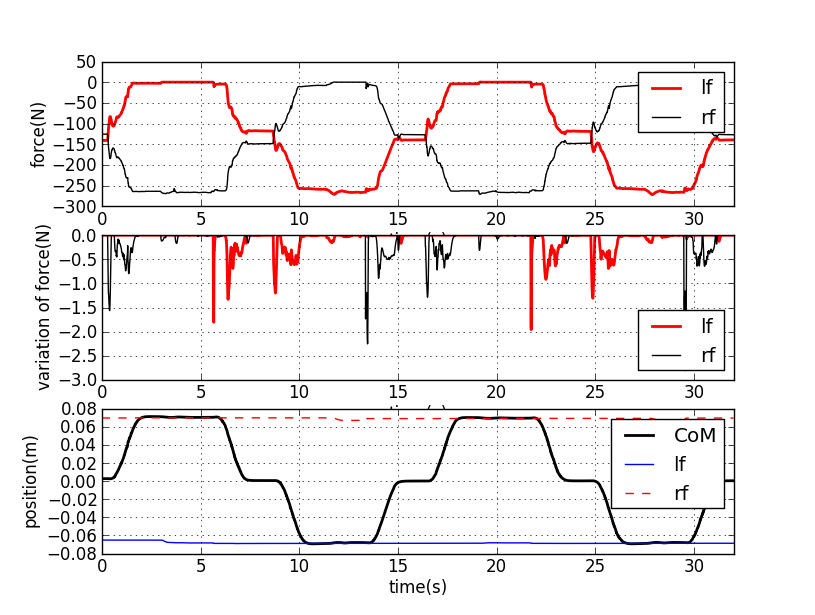
\includegraphics[width=\linewidth]{../figure/walking_force.png}
\caption{The contact forces on left foot (lf) and right foot (rf) (above), the variations of desired foot contact forces (middle), and the positions of CoM and the feet (below). The stiffness of the floor is $k=1000 N/m$, and $a$ is set to $10 Ns/m$.}
\label{walking_result}
\end{figure}
Here the CoM reference position is computed according to foot positions and desired foot contact forces.
One can obtain similar results by first defining the CoM reference trajectory, and then let controller \eqref{lqp} to find appropriate foot contact forces without adaptation to ground rigidity. This is because for a humanoid robot which is a biped, there is not much contact redundancy, and the position of the CoM largely influences the foot contact forces. However in case of contact redundancy, where not all the contact forces are dominated by the weight of the robot, it could be reasonable to first optimize all the contact forces according to environment rigidity and balance condition, and then compute the CoM target position that is compatible with the desired contact forces. 

\section{Conclusions and Future Works}
\label{Section:Conclusions}
In this paper, a reactive control approach is proposed for balancing on multiple non-rigid contacts during whole-body task execution. The contribution here is to endow existing whole-body controllers, which usually work for non-rigid environments, with the ability to adapt to unknown non-rigid environments. The goal of this adaptation is to obtain sufficient reaction forces from the environment to support the whole-body motion in a relatively natural way.

The proposed approach finds optimal robot control inputs ($\boldsymbol{\tau}$) and optimal contact forces by solving an optimization problem, which takes into account all the elementary motion task objectives, local support contact states, as well as various constraints. The solution satisfies whole-body dynamics constraint and friction cone constraints to ensure whole-body balance. 
Experiments on a simulated iCub robot are conducted to demonstrate that this approach allows the humanoid robot to maintain balance in non-rigid environments. 

One future research direction is to further study how to combine the proposed approach, which is reactive and adapts to non-rigid environments, with some motion planning techniques, which may optimize the robot motions from a global point of view, but are usually not adaptable to unknown non-rigid environments. 

Moreover, the current version of this reactive whole-body controller handles contacts for balance support. It would be interesting to extend such whole-body control by incorporating other types of elementary physical interaction tasks, such as interactions with humans through end-effector contacts. One way to achieve this goal is to apply an impedance controller, which has been applied to robotic manipulators to achieve safe and robust interactions \cite{Albu07,Yang11}, to locally control the interaction with humans.

\section*{Acknowledgment}
This work was partially supported by the European Commission, within the CoDyCo project (FP7-ICT-2011-9, No.
600716) and by the RTE company through the RTE/UPMC chair “Robotics Systems for field intervention in constrained environments” held by Vincent Padois.

\bibliographystyle{IEEEtran}
\bibliography{IEEEabrv,GHC}
\end{document}
